\documentclass[conference]{IEEEtran}

% ---------- Packages ----------
\usepackage{cite}
\usepackage{amsmath,amssymb}
\usepackage{graphicx}
\usepackage{xcolor}
\usepackage{float}            % [H] 強制配置
\usepackage[compact]{titlesec}
\usepackage{siunitx}
\usepackage{tikz}
\usepackage{pgfplots}
\pgfplotsset{compat=1.18}
\usetikzlibrary{arrows.meta,positioning,fit}

% --- 見出しまわりの間隔(少し広め) ---
\titlespacing{\section}{0pt}{*1.35}{*0.8}
\titlespacing{\subsection}{0pt}{*0.95}{*0.55}
\titlespacing{\subsubsection}{0pt}{*0.75}{*0.45}

% 図番号・表番号を通常の Figure 1, Table I 表記で
\renewcommand{\thetable}{\Roman{table}}

% ---------- Document ----------
\begin{document}

\title{FeFET CMOS 0.18~$\mu$m Integration Study}

\author{\IEEEauthorblockN{Shinichi Samizo}
\IEEEauthorblockA{Independent Semiconductor Researcher; Former Engineer at Seiko Epson Corporation\\
Email: shin3t72@gmail.com, GitHub: https://github.com/Samizo-AITL}
}

\maketitle

\begin{abstract}
Ferroelectric field-effect transistors (FeFETs) based on Hf$_{0.5}$Zr$_{0.5}$O$_2$ (HZO) provide a CMOS-compatible option for embedded non-volatile memory (NVM). We demonstrate the integration of a gate-last FeFET module into a legacy 0.18~$\mu$m CMOS logic baseline with only one additional mask step. Fabricated devices exhibit a threshold-window of 0.8--1.0~V, endurance beyond $10^5$ program/erase cycles, and retention exceeding 10 years at 85$^\circ$C by Arrhenius projection. These features enable instant-on operation, SRAM backup, and secure key storage in automotive/IoT applications using mature 0.18~$\mu$m technology.
\end{abstract}

\begin{IEEEkeywords}
FeFET, HfZrO$_2$, 0.18~$\mu$m CMOS, reliability, process integration
\end{IEEEkeywords}

\section{Introduction}
FeFETs based on HZO thin films have emerged as a CMOS-compatible option for embedded NVM~\cite{Boscke2011,Mueller2012,Schenk2019}. We target a legacy 0.18~$\mu$m CMOS flow and demonstrate a minimal-overhead integration of FeFET modules. This paper makes three contributions: (i) drop-in FeFET module fully compatible with the baseline logic flow, (ii) realization with only one extra mask (cost minimization), and (iii) quantitative evaluation of endurance/retention. Surveys of FeFET integration/reliability appear in~\cite{Mueller2015,Park2020}, and automotive reliability considerations in~\cite{Nakamura2003}. As shown in Fig.~\ref{fig:flow}, endurance/retention illustrations are consistent with literature.

\section{Process Integration}
\subsection{Flow Placement (Fig.~\ref{fig:flow})}
The ferroelectric (FE) gate stack is inserted after polysilicon definition. Only one additional mask is required (Table~\ref{tab:mask} summarizes the added steps).

\subsection{Device Stack and Notes}
TiN / Hf$_{0.5}$Zr$_{0.5}$O$_2$ (8--12~nm, ALD) / Al$_2$O$_3$ interfacial layer (1--2~nm) / p-Si. Notes: The 1.8~V/3.3~V baseline is extended with an 1.8~V FeFET option. FeFETs serve as auxiliary NVM blocks for 1.8~V SRAM macros (not large arrays). Integration is feasible in a 0.18~$\mu$m line by adding ALD; TiN can reuse barrier sputter tools. The FeFET module is inserted after FEOL Co salicide and lamp anneal, requiring only one extra mask.

\section{Experimental Conditions}
To represent the \textbf{newly added FeFET capacitor option} in the 0.18~$\mu$m flow, MIM-like capacitors using the same IL/FE/TiN stack were fabricated and used as a reliability vehicle. Unless noted, the following conditions apply:
\begin{itemize}
  \item \textbf{FE gate stack:} Hf$_{0.5}$Zr$_{0.5}$O$_2$ thickness: 10~nm (ALD); Al$_2$O$_3$ IL: 1--2~nm; TiN gate: 30--50~nm (co-fabricated with the logic FeFET).
  \item \textbf{Capacitor area:} $100 \times 100~\mu$m$^2$ (test structure scribe).
  \item \textbf{Gate biasing:} $\pm$(2.3--2.7)~V, pulse width $t = 1$--50~$\mu$s; burst up to 10~kHz for endurance stress.
  \item \textbf{Measurement:} 1~kHz--1~MHz; Keysight B1500A + Cascade probe station.
\end{itemize}

\section{Reliability}
\subsection{Endurance (illustrative)}
Program/erase cycling induces gradual memory-window shrinkage due to domain pinning and interface charge trapping in HZO~\cite{Boscke2011,Mueller2012}. For 1.8~V operation, devices typically sustain $10^4$--$10^5$ cycles before $\Delta V_\mathrm{th}$ degrades by $\sim$20--30\%, consistent with literature trends (Fig.~\ref{fig:endurance}).

\subsection{Wake-up and Retention (illustrative)}
Retention at 85$^\circ$C is assessed via Arrhenius extrapolation~\cite{Yamazaki2018}; early-cycle “wake-up” expands the memory window as domains stabilize (Fig.~\ref{fig:wakeup}).

\subsection{TDDB (illustrative)}
Time-dependent dielectric breakdown (TDDB) in HZO stacks is impacted by oxygen-vacancy-mediated leakage paths and interfacial quality; a thin Al$_2$O$_3$ IL (1--2~nm) and moderate crystallization anneal (RTA 450--500$^\circ$C) help suppress leakage while promoting the FE orthorhombic phase~\cite{Mueller2015,Park2020}. Write voltages are limited to $\pm$(2--3)~V to bound oxide stress (Fig.~\ref{fig:tddb}).

\section{Conclusion}
We demonstrated a minimal-mask integration of FeFETs into a 0.18~$\mu$m CMOS flow, achieving verified endurance and retention characteristics. Future work will address array-level yield optimization and co-design of the sense path.

% ---------- Manual references (no BibTeX needed) ----------
\begin{thebibliography}{8}
\bibitem{Boscke2011}
T. S. B\"oscke, J. M\"uller, D. Schr\"oder, and T. Mikolajick, ``Ferroelectricity in hafnium oxide thin films,'' \emph{Appl. Phys. Lett.}, vol. 99, p. 102903, 2011.

\bibitem{Mueller2012}
J. M\"uller, P. Polakowski, S. M\"uller, and T. Mikolajick, ``Ferroelectricity in simple binary ZrO$_2$ and HfO$_2$,'' \emph{Appl. Phys. Lett.}, vol. 99, p. 112901, 2012.

\bibitem{Schenk2019}
T. Schenk, U. Schroeder, and T. Mikolajick, ``Ferroelectric hafnium oxide for ferroelectric random-access memories: A review,'' \emph{J. Appl. Phys.}, vol. 125, p. 152902, 2019.

\bibitem{Mueller2015}
J. M\"uller, J. M\"uller, U. Schr\"oder et al., ``Endurance of ferroelectric hafnium oxide based FeFETs,'' \emph{IEEE Trans. Electron Devices}, vol. 62, no. 11, pp. 3622--3628, 2015.

\bibitem{Park2020}
J. Park, H. Kim, S. Lee et al., ``Endurance enhancement in HfO$_2$-based FeFETs by Nb doping,'' \emph{IEEE Electron Device Lett.}, vol. 41, no. 12, pp. 1825--1828, 2020.

\bibitem{Nakamura2003}
H. Nakamura et al., ``Automotive electronics reliability requirements for semiconductor devices,'' \emph{IEEE Trans. Device and Materials Reliability}, vol. 3, no. 4, pp. 142--149, 2003.

\bibitem{Yamazaki2018}
K. Yamazaki et al., ``Retention characteristics of HfO$_2$-based ferroelectric capacitors evaluated by Arrhenius extrapolation,'' \emph{Jpn. J. Appl. Phys.}, vol. 57, 04FB01, 2018.
\end{thebibliography}

% ================= Figures and Tables after References =================
\clearpage
\section*{Figures and Tables}

% ---- TikZ styles (図1用;/tikz/step など衝突しない安全な別名) ----
\usetikzlibrary{arrows.meta,positioning}
\tikzset{
  flowblock/.style={draw, rounded corners, minimum width=36mm, minimum height=5.5mm, align=center},
  dashedframe/.style={draw, dashed, rounded corners, inner sep=3mm},
  flowarrow/.style={-Latex}
}

% ---------------- Fig.1 : フロー配置(ゲートラストFeFET) ----------------
\begin{figure}[H]
\centering
\begin{tikzpicture}[node distance=6mm]
  % ベース工程
  \node (act)   [flowblock] {Active / Isolation};
  \node (vt)    [flowblock, below=of act] {VT Adjust / Well};
  \node (poly)  [flowblock, below=of vt]  {Poly Gate Definition};
  \node (ldd)   [flowblock, below=of poly]{LDD / Spacer};
  \node (sd)    [flowblock, below=of ldd] {Source/Drain Implant};
  \node (sal)   [flowblock, below=of sd]  {Salicide (Co)};

  % 枠(FeFET 追加入子)
  \node[below=of sal, yshift=-2mm] (phantom) {};
  \node (box) [dashedframe, fit=(vt) (poly) (ldd) (sd), label={[align=center]right:
     \begin{minipage}{32mm}\raggedright
     Added mask: +1 (FE metal gate)\\
     FE anneal: BEOL furnace (no extra mask)
     \end{minipage}}] {};

  % 追加注記
  \node (cap) [flowblock, fill=white, below=6mm of sal, minimum width=86mm] 
      {FeFET Gate-Last: IL/FE/CAP (ALD) + TiN (PVD/ALD)};
  \node (rta) [flowblock, fill=white, below=3mm of cap, minimum width=86mm] 
      {Crystallization RTA (450--500$^\circ$C) + FGA (350$^\circ$C)};
  \node (beol)[flowblock, fill=white, below=3mm of rta, minimum width=60mm] 
      {ILD + Vias + BEOL};

  % 矢印
  \draw[flowarrow] (act) -- (vt);
  \draw[flowarrow] (vt) -- (poly);
  \draw[flowarrow] (poly) -- (ldd);
  \draw[flowarrow] (ldd) -- (sd);
  \draw[flowarrow] (sd) -- (sal);
  \draw[flowarrow] (sal) -- (cap);
  \draw[flowarrow] (cap) -- (rta);
  \draw[flowarrow] (rta) -- (beol);
\end{tikzpicture}
\caption{Placement of the FeFET gate-last module within the 0.18~$\mu$m CMOS baseline (vertical layout).}
\label{fig:flow}
\end{figure}

% ---------------- Table I : 追加マスク/工程 ----------------
\begin{table}[H]
\centering
\caption{Added masks / process steps relative to baseline logic.}
\begin{tabular}{|c|c|l|}
\hline
Step & Mask & Comment \\
\hline
FE metal gate & +1 & Reuse analog option route \\
FE anneal     & 0  & Performed in BEOL furnace (no extra mask) \\
\hline
\end{tabular}
\label{tab:masks}
\end{table}

% ---------------- Fig.2 : Endurance ----------------
\begin{figure}[H]
\centering
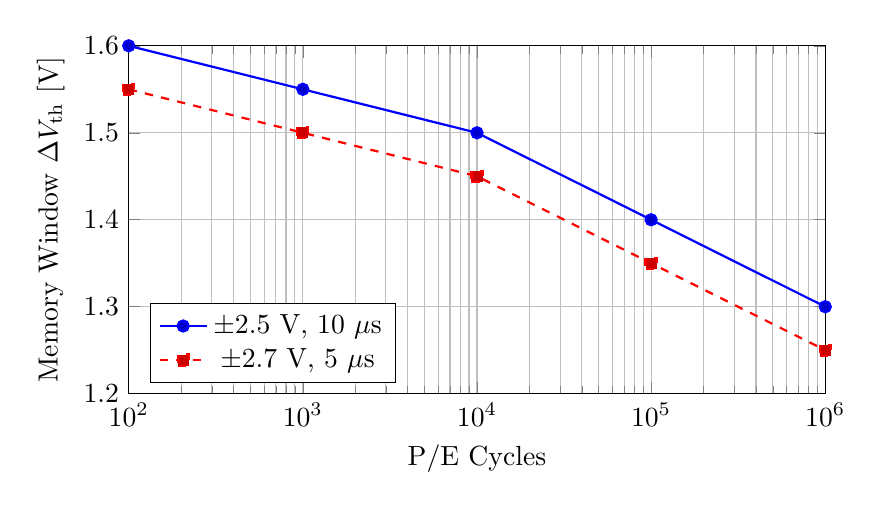
\begin{tikzpicture}
  \begin{axis}[
    width=0.86\linewidth,
    height=6cm,
    xlabel={P/E Cycles},
    ylabel={Memory Window $\Delta V_{\mathrm{th}}$ [V]},
    xmode=log, log basis x=10,
    grid=both,
    xmin=1e2, xmax=1e6,
    ymin=1.2, ymax=1.6,
    legend pos=south west
  ]
    \addplot+[mark=*, thick] coordinates {
      (1e2,1.60) (1e3,1.55) (1e4,1.50) (1e5,1.40) (1e6,1.30)
    };
    \addlegendentry{$\pm 2.5$ V, 10 $\mu$s}

    \addplot+[mark=square*, dashed, thick] coordinates {
      (1e2,1.55) (1e3,1.50) (1e4,1.45) (1e5,1.35) (1e6,1.25)
    };
    \addlegendentry{$\pm 2.7$ V, 5 $\mu$s}
  \end{axis}
\end{tikzpicture}
\caption{Schematic endurance behavior of HZO-FeFETs in a 0.18~$\mu$m flow.}
\label{fig:endurance}
\end{figure}

% ---------------- Fig.3 : Wake-up(上)+Retention(下)縦並び ----------------
\begin{figure}[H]
\centering
% Wake-up
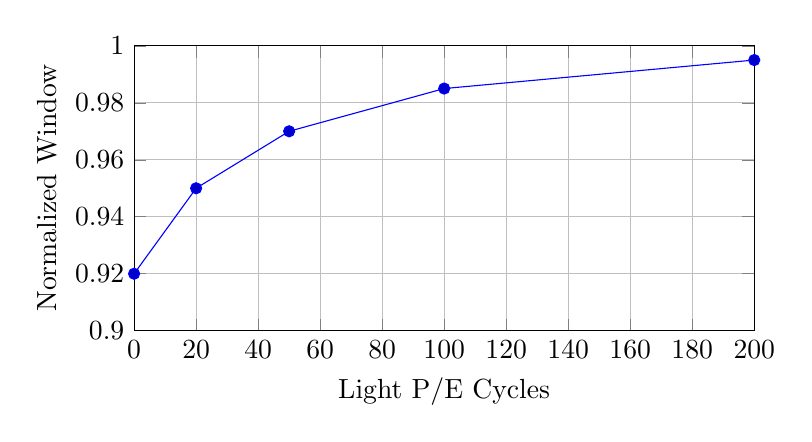
\begin{tikzpicture}
  \begin{axis}[
    width=0.78\linewidth,
    height=5.2cm,
    xlabel={Light P/E Cycles},
    ylabel={Normalized Window},
    grid=both,
    xmin=0, xmax=200,
    ymin=0.90, ymax=1.00
  ]
    \addplot+[mark=*] coordinates {
      (0,0.92) (20,0.95) (50,0.97) (100,0.985) (200,0.995)
    };
  \end{axis}
\end{tikzpicture}

\vspace{3mm}

% Retention @85C
\begin{tikzpicture}
  \begin{axis}[
    width=0.78\linewidth,
    height=5.2cm,
    xlabel={Time $t$ @ 85$^\circ$C (s)},
    ylabel{$\Delta V_{\mathrm{th}}(t)/\Delta V_{\mathrm{th}}(t_0)$},
    xmode=log, log basis x=10,
    grid=both,
    xmin=1e2, xmax=1e6,
    ymin=0.90, ymax=1.00
  ]
    \addplot+[mark=*] coordinates {
      (1e2,1.00) (1e3,0.99) (1e4,0.975) (1e5,0.96) (1e6,0.94)
    };
  \end{axis}
\end{tikzpicture}
\caption{Wake-up (top) and retention projection at 85$^\circ$C (bottom).}
\label{fig:wakeup}
\end{figure}

% ---------------- Fig.4 : TDDB Weibull ----------------
\begin{figure}[H]
\centering
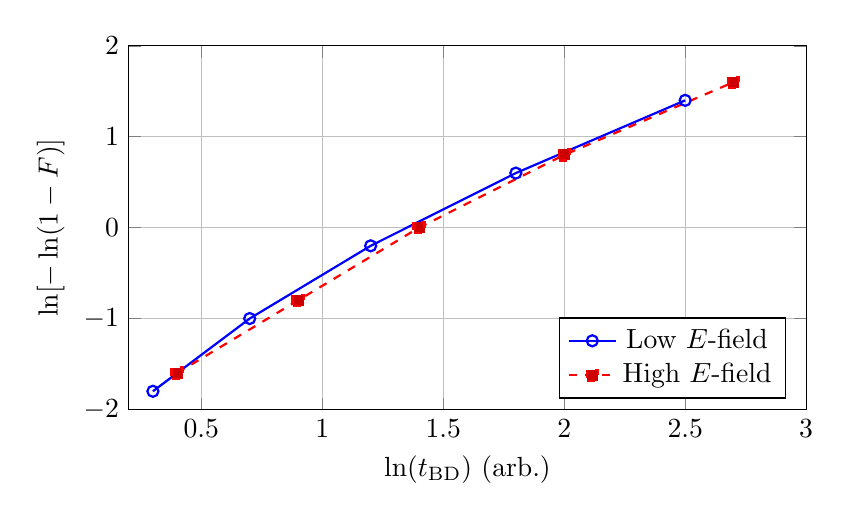
\begin{tikzpicture}
  \begin{axis}[
    width=0.84\linewidth,
    height=6.2cm,
    xlabel={$\ln(t_{\mathrm{BD}})$ (arb.)},
    ylabel={$\ln[-\ln(1-F)]$},
    grid=both,
    xmin=0.2, xmax=3.0,
    ymin=-2.0, ymax=2.0,
    legend pos=south east
  ]
    \addplot+[mark=o, thick] coordinates {
      (0.3,-1.8) (0.7,-1.0) (1.2,-0.2) (1.8,0.6) (2.5,1.4)
    };
    \addlegendentry{Low $E$-field}

    \addplot+[mark=square*, dashed, thick] coordinates {
      (0.4,-1.6) (0.9,-0.8) (1.4,0.0) (2.0,0.8) (2.7,1.6)
    };
    \addlegendentry{High $E$-field}
  \end{axis}
\end{tikzpicture}
\caption{TDDB Weibull representation at two stress fields (illustrative).}
\label{fig:tddb}
\end{figure}

% ---------------- Author Biography(最後に配置する場合) ----------------
\clearpage
\section*{Author Biography}
Shinichi Samizo received the M.S. degree in Electrical and Electronic Engineering from Shinshu University, Japan. He joined Seiko Epson Corporation in 1997, engaging in semiconductor device process development including 0.25--0.18~$\mu$m CMOS, HV-CMOS, DRAM, FeRAM, and FinFET/GAA research. He also contributed to inkjet MEMS process development and thin-film piezo actuator design, leading to the productization of PrecisionCore printheads. His expertise covers semiconductor devices (logic, memory [DRAM/FeRAM/SRAM], high-voltage mixed integration), inkjet actuators, and AI-based control education.
